%! TeX program = pdflatex
%! BIB program = biber
% =========================================================================
% MASTER FILE: PROPOSAL SEMINAR PROPOSAL (SEMPRO)
% Departemen Teknologi Kedokteran - Fakultas Kedokteran dan Kesehatan ITS
% Mengacu pada SK Rektor ITS No. 280/IT2/T/HK.00.01/2022
% =========================================================================

\newcommand{\doctypename}{PROPOSAL TUGAS AKHIR}
\newcommand{\engdoctypename}{FINAL PROJECT PROPOSAL}

% Judul dokumen
\title{Proposal Tugas Akhir (Sempro) ITS - Teknologi Kedokteran}
\author{\name}

% Pengaturan ukuran teks dan bentuk halaman satu sisi untuk Proposal
\documentclass[12pt,oneside]{report}

% Pengaturan ukuran halaman dan margin (Sesuai Pedoman ITS: Atas 3cm, Kiri 3cm, Kanan 2cm, Bawah 2.5cm)
\usepackage[a4paper,top=30mm,left=30mm,right=20mm,bottom=25mm]{geometry}

% Pengaturan ukuran spasi (1 / singlespacing)
\usepackage[singlespacing]{setspace}

% Pengaturan detail pada file PDF
\usepackage[pdfauthor={\@author},bookmarksnumbered,pdfborder={0 0 0}]{hyperref}

% Pengaturan jenis karakter
\usepackage[utf8]{inputenc}
\usepackage[T1]{fontenc}

% Pengaturan pewarnaan
\usepackage[table,xcdraw]{xcolor}

% Pengaturan kutipan artikel
\usepackage[style=apa, backend=biber]{biblatex}

% Package lainnya
\usepackage{changepage}
\usepackage{enumitem}
\usepackage{eso-pic}
\usepackage{txfonts} % Font times
\usepackage{etoolbox}
\usepackage{graphicx}
\usepackage{lipsum}
\usepackage{longtable}
\usepackage{tabularx}
\usepackage{wrapfig}
\usepackage{float}

% Pengaturan penomoran halaman (kanan bawah sesuai pedoman ITS Subbab 3.2.f)
\usepackage{fancyhdr}
\fancyhf{}
\renewcommand{\headrulewidth}{0pt}
\pagestyle{fancy}
\fancyfoot[R]{\thepage}
\patchcmd{\chapter}{plain}{fancy}{}{}
\patchcmd{\chapter}{empty}{plain}{}{}

% Command untuk bulan
\newcommand{\MONTH}{%
  \ifcase\the\month
  \or Januari% 1
  \or Februari% 2
  \or Maret% 3
  \or April% 4
  \or Mei% 5
  \or Juni% 6
  \or Juli% 7
  \or Agustus% 8
  \or September% 9
  \or Oktober% 10
  \or November% 11
  \or Desember% 12
  \fi}
\newcommand{\ENGMONTH}{%
  \ifcase\the\month
  \or January% 1
  \or February% 2
  \or March% 3
  \or April% 4
  \or May% 5
  \or June% 6
  \or July% 7
  \or August% 8
  \or September% 9
  \or October% 10
  \or November% 11
  \or December% 12
  \fi}

% Pengaturan format judul bab (sebaris: BAB I PENDAHULUAN dengan 1 spasi biasa)
\usepackage{titlesec}
\titleformat{\chapter}[block]{\bfseries\Large\centering}{BAB \Roman{chapter}\ }{0pt}{}
\titleformat{\section}{\bfseries\large}{\MakeUppercase{\thesection}}{1ex}{\vspace{1ex}}
\titleformat{\subsection}{\bfseries\large}{\MakeUppercase{\thesubsection}}{1ex}{}
\titleformat{\subsubsection}{\bfseries\large}{\MakeUppercase{\thesubsubsection}}{1ex}{}
\titlespacing{\chapter}{0ex}{0ex}{3ex}
\titlespacing{\section}{0ex}{1ex}{0ex}
\titlespacing{\subsection}{0ex}{0.5ex}{0ex}
\titlespacing{\subsubsection}{0ex}{0.5ex}{0ex}

% =========================================================================
% Variabel Dokumen - Template Proposal & Buku Tugas Akhir
% Departemen Teknologi Kedokteran - Fakultas Kedokteran dan Kesehatan ITS
% =========================================================================
% Petunjuk: Sesuaikan variabel di bawah ini dengan data Anda masing-masing.

% -------------------------------------------------------------------------
% 1. IDENTITAS MAHASISWA
% -------------------------------------------------------------------------
\newcommand{\name}{Nama Lengkap Mahasiswa}
\newcommand{\authorname}{Nama Belakang, Nama Depan}
\newcommand{\nickname}{Nama Panggilan}
\newcommand{\nrp}{5049231XXX}

% -------------------------------------------------------------------------
% 2. DOSEN PEMBIMBING & PENGUJI
% -------------------------------------------------------------------------
\newcommand{\advisor}{Nama Pembimbing Utama, Gelar}
\newcommand{\advisornip}{NIP/NPP Dosen Pembimbing Utama}

\newcommand{\coadvisor}{Nama Pembimbing Pendamping, Gelar}
\newcommand{\coadvisornip}{NIP/NPP Dosen Pembimbing Pendamping}

% Tim Penguji (Diisi saat ujian Tugas Akhir / Sidang, beri tanda '-' jika belum ada)
\newcommand{\examinerone}{-}
\newcommand{\examineronenip}{-}
\newcommand{\examinertwo}{-}
\newcommand{\examinertwonip}{-}
\newcommand{\examinerthree}{-}
\newcommand{\examinerthreenip}{-}

\newcommand{\headofdepartment}{Nama Kepala Departemen, Gelar}
\newcommand{\headofdepartmentnip}{NIP/NPP Kepala Departemen}

% -------------------------------------------------------------------------
% 3. JUDUL TUGAS AKHIR / PROPOSAL
% -------------------------------------------------------------------------
\newcommand{\tatitle}{JUDUL PROPOSAL/TUGAS AKHIR DITULIS SINGKAT, JELAS DAN MENGGAMBARKAN TEMA POKOK}
\newcommand{\engtatitle}{THE TITLE OF THE FINAL PROJECT PROPOSAL IS WRITTEN BRIEFLY, CLEARLY AND DESCRIBING THE MAIN THEME}

% -------------------------------------------------------------------------
% 4. TEMPAT DAN TAHUN
% -------------------------------------------------------------------------
\newcommand{\place}{Surabaya}

% -------------------------------------------------------------------------
% 5. PROGRAM STUDI & DEPARTEMEN (Khusus Teknologi Kedokteran ITS)
% -------------------------------------------------------------------------
\newcommand{\studyprogram}{Teknologi Kedokteran}
\newcommand{\engstudyprogram}{Medical Technology}

\newcommand{\department}{Teknologi Kedokteran}
\newcommand{\engdepartment}{Medical Technology}

% -------------------------------------------------------------------------
% 6. FAKULTAS (Fakultas Kedokteran dan Kesehatan ITS)
% -------------------------------------------------------------------------
\newcommand{\faculty}{Kedokteran dan Kesehatan}
\newcommand{\engfaculty}{Medicine and Health}

\newcommand{\facultyshort}{FKK}
\newcommand{\engfacultyshort}{FMH}

% -------------------------------------------------------------------------
% 7. GELAR AKADEMIK (Sarjana Teknik / Bachelor of Engineering)
% -------------------------------------------------------------------------
\newcommand{\degree}{Sarjana Teknik}
\newcommand{\engdegree}{Bachelor of Engineering}

% -------------------------------------------------------------------------
% 8. KODE MATA KULIAH PROPOSAL / TUGAS AKHIR TEKNOLOGI KEDOKTERAN
% -------------------------------------------------------------------------
% Kode Proposal Tugas Akhir: KT234801
\newcommand{\coursecode}{KT234801}


% Tambahkan format tanda hubung yang benar di sini
\hyphenation{
  ro-ket
  me-ngem-bang-kan
  per-hi-tu-ngan
  tek-no-lo-gi
  me-la-ku-kan
  ber-so-si-al-i-sa-si
}

% Menambahkan resource daftar pustaka
\addbibresource{pustaka/pustaka.bib}

% Pengaturan format potongan kode
\usepackage{listings}
\definecolor{comment}{RGB}{0,128,0}
\definecolor{string}{RGB}{255,0,0}
\definecolor{keyword}{RGB}{0,0,255}
\lstdefinestyle{codestyle}{
  commentstyle=\color{comment},
  stringstyle=\color{string},
  keywordstyle=\color{keyword},
  basicstyle=\footnotesize\ttfamily,
  numbers=left,
  numberstyle=\tiny,
  numbersep=5pt,
  frame=lines,
  breaklines=true,
  prebreak=\raisebox{0ex}[0ex][0ex]{\ensuremath{\hookleftarrow}},
  showstringspaces=false,
  upquote=true,
  tabsize=2,
}
\lstset{style=codestyle}

% Isi keseluruhan dokumen Proposal
\begin{document}

% =========================================================================
% HALAMAN SAMPUL PROPOSAL (Mengikuti format Tekdok - Acuan Tegar)
% 1. Sampul Luar Biru
% 2. Sampul Dalam Bahasa Indonesia (Pita Biru 10 mm)
% 3. Sampul Dalam Bahasa Inggris (Pita Biru 10 mm)
% =========================================================================
% Sampul Luar Biru
\newcommand\covercontents{sampul/konten-id.tex}
\AddToShipoutPictureBG*{
  \AtPageLowerLeft{
    % Ubah nilai berikut jika posisi horizontal background tidak sesuai
    \hspace{-3.25mm}

    % Ubah nilai berikut jika posisi vertikal background tidak sesuai
    \raisebox{0mm}{
      
\includegraphics[width=\paperwidth,height=\paperheight]{sampul/gambar/sampul-luar.png}
    }
  }
}

% Menyembunyikan nomor halaman
\thispagestyle{empty}

% Pengaturan margin untuk menyesuaikan konten sampul
\newgeometry{
  top=55mm,
  left=30mm,
  right=20mm,
  bottom=20mm
}

\begin{flushleft}

  % Pemilihan font sans serif
  \sffamily

  % Pemilihan warna font putih
  \color{white}

  % Pemilihan font bold
  \fontseries{bx}
  \selectfont
  \begin{spacing}{1.5}
    \input{\covercontents}
  \end{spacing}

\end{flushleft}

\restoregeometry

\clearpage

% Sampul Dalam Bahasa Indonesia
\renewcommand\covercontents{sampul/konten-id.tex}
\AddToShipoutPictureBG*{
  \AtPageLowerLeft{
    % Ubah nilai berikut jika posisi horizontal background tidak sesuai
    \hspace{-4mm}

    % Ubah nilai berikut jika posisi vertikal background tidak sesuai
    \raisebox{0mm}{
      
\includegraphics[width=\paperwidth,height=\paperheight]{sampul/gambar/sampul-luar-tipis.png}
    }
  }
}

% Menyembunyikan nomor halaman
\thispagestyle{empty}

% Pengaturan margin untuk menyesuaikan konten sampul
\newgeometry{
  top=65mm,
  left=30mm,
  right=30mm,
  bottom=20mm
}

\begin{flushleft}

  % Pemilihan font sans serif
  \sffamily

  % Pemilihan font bold
  \fontseries{bx}
  \selectfont
  \begin{spacing}{1.5}
    \input{\covercontents}
  \end{spacing}

\end{flushleft}

\restoregeometry

\clearpage

% Sampul Dalam Bahasa Inggris
\renewcommand\covercontents{sampul/konten-en.tex}
\AddToShipoutPictureBG*{
  \AtPageLowerLeft{
    % Ubah nilai berikut jika posisi horizontal background tidak sesuai
    \hspace{-4mm}

    % Ubah nilai berikut jika posisi vertikal background tidak sesuai
    \raisebox{0mm}{
      
\includegraphics[width=\paperwidth,height=\paperheight]{sampul/gambar/sampul-luar-tipis.png}
    }
  }
}

% Menyembunyikan nomor halaman
\thispagestyle{empty}

% Pengaturan margin untuk menyesuaikan konten sampul
\newgeometry{
  top=65mm,
  left=30mm,
  right=30mm,
  bottom=20mm
}

\begin{flushleft}

  % Pemilihan font sans serif
  \sffamily

  % Pemilihan font bold
  \fontseries{bx}
  \selectfont
  \begin{spacing}{1.5}
    \input{\covercontents}
  \end{spacing}

\end{flushleft}

\restoregeometry

\clearpage

% =========================================================================
% PENOMORAN HALAMAN BAGIAN AWAL (Sesuai Pedoman ITS Subbab 2.1 & 3.2.f)
% Diberi nomor halaman angka Romawi kecil (i, ii, iii, dst.) di kanan bawah.
% Dimulai dari Lembar Pengesahan.
% =========================================================================
\pagenumbering{roman}
\setcounter{page}{1}

% Label tabel dan gambar dalam bahasa indonesia
\renewcommand{\figurename}{Gambar}
\renewcommand{\tablename}{Tabel}

% Pengaturan format caption (tebal Gambar X.X., titik, dan jarak rapat ke gambar)
\makeatletter
\setlength{\abovecaptionskip}{3pt}
\setlength{\belowcaptionskip}{0pt}
\long\def\@makecaption#1#2{%
  \vskip\abovecaptionskip
  \sbox\@tempboxa{\textbf{#1.} #2}%
  \ifdim \wd\@tempboxa >\hsize
    \textbf{#1.} #2\par
  \else
    \global \@minipagefalse
    \hb@xt@\hsize{\hfil\box\@tempboxa\hfil}%
  \fi
  \vskip\belowcaptionskip}
\makeatother

% Pengaturan ukuran indentasi paragraf
\setlength{\parindent}{2em}

% Pengaturan ukuran spasi paragraf
\setlength{\parskip}{1ex}

% Lembar pengesahan Bahasa Indonesia (Lampiran 2)
\begin{center}
  \large
  \textbf{LEMBAR PENGESAHAN}
\end{center}

\begin{center}
  \textbf{\tatitle{}}
\end{center}

\begingroup
% Pemilihan font ukuran small
\small

\begin{center}
  \textbf{\doctypename{}}
  \\Diajukan untuk memenuhi salah satu syarat \\
  memperoleh gelar \degree{} pada \\
  Program Studi S-1 \studyprogram{} \\
  Fakultas \faculty{} \\
  Institut Teknologi Sepuluh Nopember
\end{center}

\begin{center}
  Oleh : \textbf{\name{}}
  \\NRP. \nrp{}
\end{center}

\begin{center}
  Disetujui oleh Tim Penguji \doctypename{} :
\end{center}

\begingroup
% Menghilangkan padding
\setlength{\tabcolsep}{0pt}

\noindent
\begin{tabularx}{\textwidth}{X l}
  1. \advisor{}               & Pembimbing                          \\
  \hspace*{1.5em}NIP. \advisornip{}       &                                     \\
                              & ................................... \\
                              &                                     \\
  2. \coadvisor{}             & Ko-pembimbing                       \\
  \hspace*{1.5em}NIP. \coadvisornip{}     &                                     \\
                              & ................................... \\
                              &                                     \\
  3. \examinerone{}           & Penguji                             \\
  \hspace*{1.5em}NIP. \examineronenip{}   &                                     \\
                              & ................................... \\
\end{tabularx}
\endgroup

\vfill

\begin{center}
  \textbf{\MakeUppercase{\place{}}\\\MONTH{}, \the\year{}}
\end{center}
\endgroup


\clearpage

% Lembar pengesahan Bahasa Inggris (Approval Sheet - Lampiran 2)
\begin{center}
  \large
  \textbf{APPROVAL SHEET}
\end{center}

\begin{center}
  \textbf{\engtatitle{}}
\end{center}

\begingroup
% Pemilihan font ukuran small
\small

\begin{center}
  \textbf{\engdoctypename{}}
  \\Submitted to fulfill one of the requirements \\
  for obtaining a degree \engdegree{} at \\
  Undergraduate Study Program of \engstudyprogram{} \\
  Faculty of \engfaculty{} \\
  Institut Teknologi Sepuluh Nopember
\end{center}

\begin{center}
  By: \textbf{\name{}}
  \\NRP. \nrp{}
\end{center}

\begin{center}
  Approved by \engdoctypename{} Examiner Team:
\end{center}

\begingroup
% Menghilangkan padding
\setlength{\tabcolsep}{0pt}

\noindent
\begin{tabularx}{\textwidth}{X l}
  1. \advisor{}               & Advisor                             \\
  \hspace*{1.5em}NIP. \advisornip{}       &                                     \\
                              & ................................... \\
                              &                                     \\
  2. \coadvisor{}             & Co-Advisor                          \\
  \hspace*{1.5em}NIP. \coadvisornip{}     &                                     \\
                              & ................................... \\
                              &                                     \\
  3. \examinerone{}           & Examiner                            \\
  \hspace*{1.5em}NIP. \examineronenip{}   &                                     \\
                              & ................................... \\
\end{tabularx}
\endgroup

\vfill

\begin{center}
  \textbf{\MakeUppercase{\place{}}\\\ENGMONTH{}, \the\year{}}
\end{center}
\endgroup


\clearpage

% Abstrak Bahasa Indonesia
\begin{center}
  \large\textbf{ABSTRAK}
\end{center}

\addcontentsline{toc}{chapter}{ABSTRAK}

\begin{center}
  \textbf{\tatitle{}}
\end{center}

\vspace{1ex}

\begingroup
\setlength{\tabcolsep}{0pt}

\noindent
\begin{tabularx}{\textwidth}{l >{\centering}m{2em} X}
  Nama Mahasiswa / NRP & : & \name{} / \nrp{} \\
  Departemen           & : & \department{} \facultyshort{} - ITS \\
  Dosen Pembimbing     & : & 1. \advisor{} \\
                       &   & 2. \coadvisor{} \\
\end{tabularx}
\endgroup

\vspace{2ex}

\noindent\textbf{Abstrak}

% Ubah paragraf berikut dengan abstrak dari proposal tugas akhir
Pada penelitian ini diajukan \lipsum[1]

\vspace{2ex}

\noindent\textbf{Kata kunci:} Edge AI, \emph{Speech-to-Text}, SLM, SOAP, Rekam Medis.


\clearpage

% Abstrak Bahasa Inggris
\begin{center}
  \large\textbf{ABSTRACT}
\end{center}

\addcontentsline{toc}{chapter}{ABSTRACT}

\begin{center}
  \textbf{\engtatitle{}}
\end{center}

\vspace{1ex}

\begingroup
\setlength{\tabcolsep}{0pt}

\noindent
\begin{tabularx}{\textwidth}{l >{\centering}m{2em} X}
  Student Name / NRP & : & \name{} / \nrp{} \\
  Department         & : & \engdepartment{} \engfacultyshort{} - ITS \\
  Advisor            & : & 1. \advisor{} \\
                     &   & 2. \coadvisor{} \\
\end{tabularx}
\endgroup

\vspace{2ex}

\noindent\textbf{Abstract}

% Ubah paragraf berikut dengan abstrak dari proposal tugas akhir dalam Bahasa Inggris
\emph{\lipsum[1]}

\vspace{2ex}

\noindent\textbf{Keywords:} keyword 1, keyword 2, keyword 3, keyword 4, keyword 5.


\clearpage

% Daftar isi
\renewcommand*\contentsname{DAFTAR ISI}
\addcontentsline{toc}{chapter}{\contentsname}
\tableofcontents
\clearpage

% Daftar gambar
\renewcommand*\listfigurename{DAFTAR GAMBAR}
\addcontentsline{toc}{chapter}{\listfigurename}
\listoffigures
\clearpage

% Daftar tabel
\renewcommand*\listtablename{DAFTAR TABEL}
\addcontentsline{toc}{chapter}{\listtablename}
\listoftables
\clearpage

% Nomor halaman isi dimulai dari sini (angka Arab 1 di kanan bawah)
\pagenumbering{arabic}

% Bab 1 Pendahuluan
%! TeX root = ../main.tex
\chapter{PENDAHULUAN}
\label{chap:pendahuluan}

\section{Latar Belakang}
\label{sec:latarbelakang}

\lipsum[1-2]

\section{Rumusan Masalah}
\label{sec:rumusanmasalah}

Berdasarkan latar belakang yang telah diuraikan, rumusan masalah dalam penelitian ini adalah:
\begin{enumerate}
  \item Bagaimana \lipsum[1][1-2]
  \item Bagaimana \lipsum[2][1-2]
\end{enumerate}

\section{Batasan Masalah}
\label{sec:batasanmasalah}

Batasan masalah dalam penelitian ini adalah sebagai berikut:
\begin{enumerate}
  \item \lipsum[3][1-2]
  \item \lipsum[4][1-2]
\end{enumerate}

\section{Tujuan}
\label{sec:tujuan}

Tujuan yang ingin dicapai dari penelitian ini adalah:
\begin{enumerate}
  \item \lipsum[1][1-2]
  \item \lipsum[2][1-2]
\end{enumerate}

\section{Manfaat}
\label{sec:manfaat}

Manfaat yang diharapkan dari hasil penelitian ini antara lain:
\begin{enumerate}
  \item \textbf{Bagi Peneliti dan Akademisi}: \lipsum[1][1-3]
  \item \textbf{Bagi Sektor Kesehatan/Klinis}: \lipsum[2][1-3]
\end{enumerate}


\clearpage

% Bab 2 Tinjauan Pustaka
%! TeX root = ../main.tex
\chapter{TINJAUAN PUSTAKA}
\label{chap:tinjauanpustaka}

\section{Hasil Penelitian Terdahulu}
\label{sec:penelitianterdahulu}

Pada bagian ini dijelaskan kajian dari penelitian-penelitian terdahulu yang relevan dengan topik tugas akhir. Perkembangan teknologi kecerdasan buatan dalam bidang kesehatan telah berkembang secara pesat dalam mendukung efisiensi pelayanan klinis \parencite{rajpurkar2022ai}.

\lipsum[1]

\section{Dasar Teori}
\label{sec:dasarteori}

Bagian ini memuat teori-teori dasar, konsep, dan algoritma yang melandasi penelitian.

\subsection{Teori Pendukung Pertama}
\label{subsec:teoripertama}

\lipsum[2]

\begin{equation}
  \label{eq:persamaan1}
  \sum \mathbf{F} = 0\; \Leftrightarrow\; \frac{\mathrm{d} \mathbf{v} }{\mathrm{d}t} = 0
\end{equation}

\subsection{Teori Pendukung Kedua}
\label{subsec:teorikedua}

\lipsum[3]

\clearpage

% Bab 3 Metodologi (memuat rencana jadwal kegiatan Lampiran 5)
%! TeX root = ../main.tex
\chapter{METODOLOGI}
\label{chap:metodologi}

% Ubah bagian ini sesuai dengan metodologi penelitian proposal / tugas akhir Anda.

\section{Diagram Alir Penelitian}
\label{sec:diagramalir}

Metodologi penelitian ini dilakukan melalui tahapan sebagaimana ditunjukkan pada Gambar~\ref{fig:alir-metodologi}. \lipsum[1]

\begin{figure}[H]
  \centering
  % Ganti berkas gambar berikut dengan diagram alir penelitian Anda di folder gambar/
  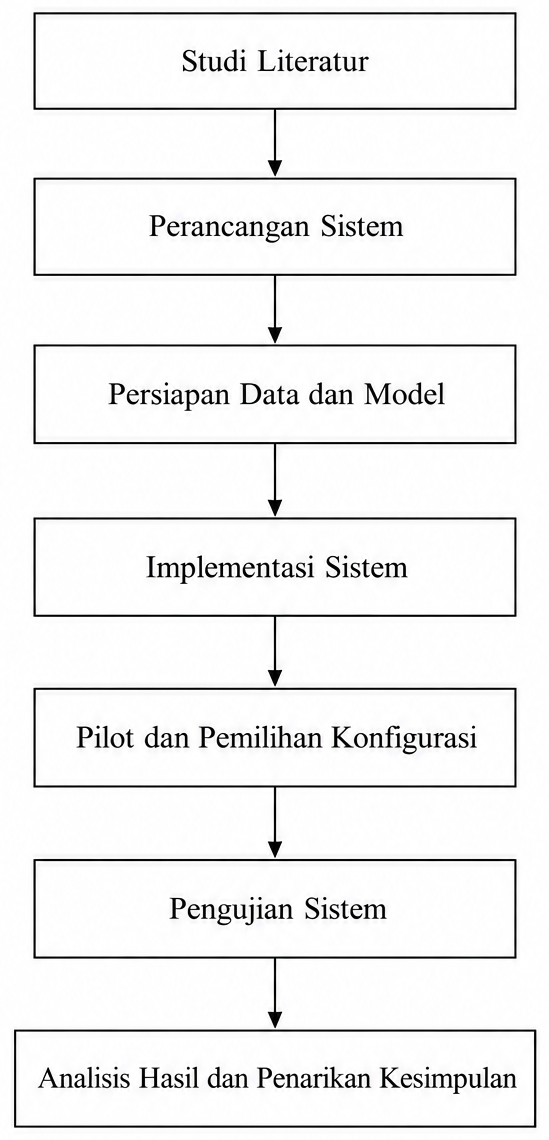
\includegraphics[height=12cm]{gambar/gambar-3-1.png}
  \caption{Diagram Alir Metodologi Penelitian}
  \label{fig:alir-metodologi}
\end{figure}

\section{Bahan dan Peralatan}
\label{sec:bahanperalatan}

Pada bagian ini diuraikan bahan, spesifikasi peralatan, perangkat keras (\emph{hardware}), dan perangkat lunak (\emph{software}) yang digunakan dalam penelitian.

\lipsum[2]

\begin{enumerate}
  \item \textbf{Perangkat Keras}: \lipsum[3][1-2]
  \item \textbf{Perangkat Lunak}: \lipsum[4][1-2]
\end{enumerate}

\section{Perancangan Sistem}
\label{sec:perancangansistem}

\subsection{Arsitektur dan Diagram Blok Sistem}
\label{subsec:arsitektursistem}

Sistem dirancang dengan alur kerja yang menghubungkan setiap modul dari akuisisi data, prapemrosesan, pemrosesan utama, hingga keluaran atau tampilan antarmuka. Hubungan antarblok sistem dan aliran data ditunjukkan pada Gambar~\ref{fig:blok-sistem}.

\begin{figure}[H]
  \centering
  % Ganti berkas gambar berikut dengan diagram blok sistem Anda di folder gambar/
  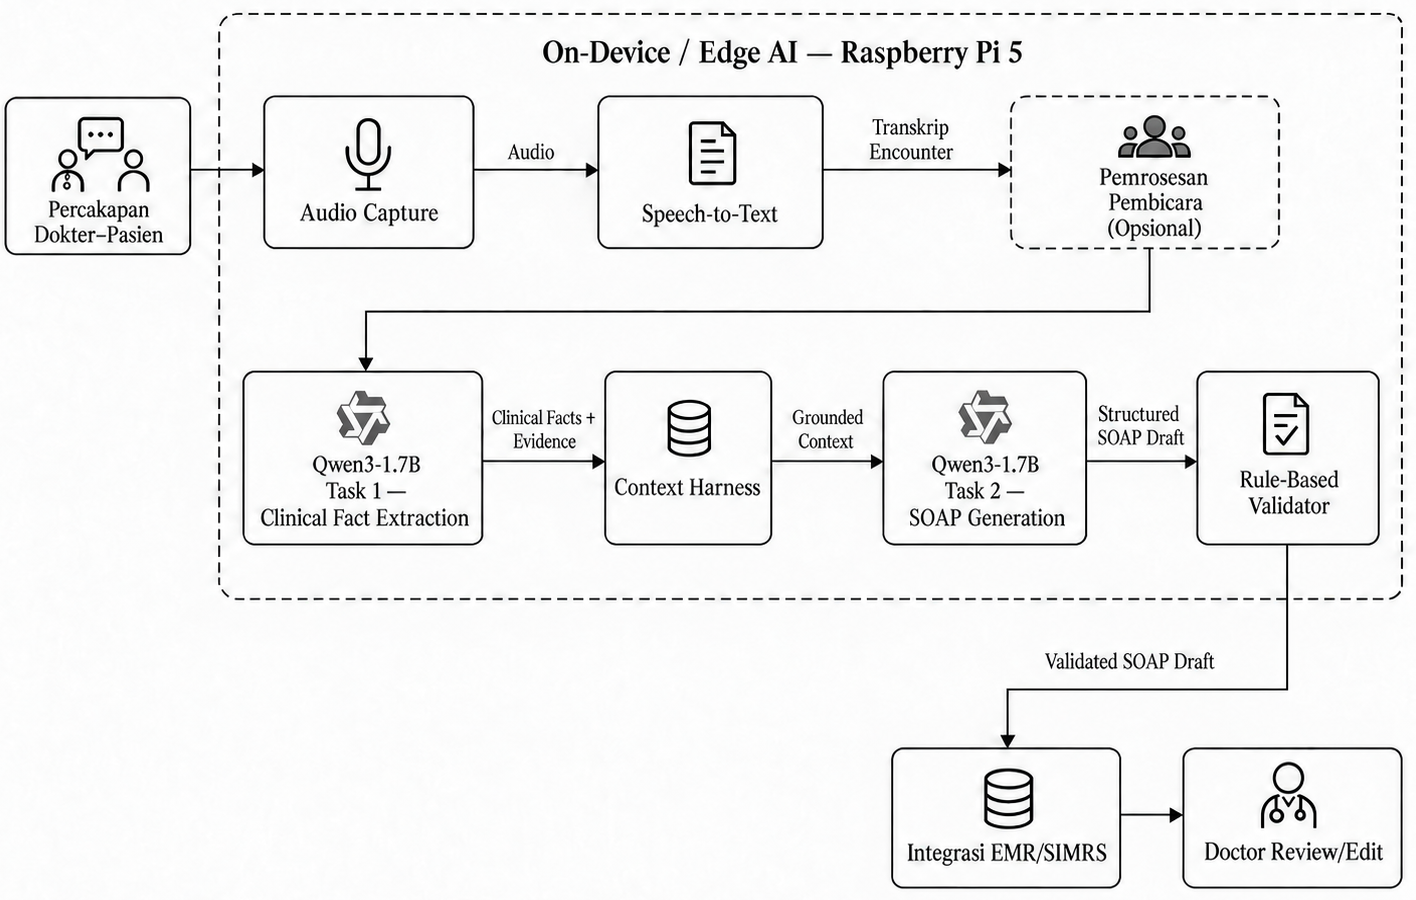
\includegraphics[width=0.9\textwidth]{gambar/gambar-3-2.png}
  \caption{Diagram Blok Sistem}
  \label{fig:blok-sistem}
\end{figure}

\subsection{Tahapan Implementasi}
\label{subsec:tahapanimplementasi}

\lipsum[5-6]

\section{Prosedur Pengujian dan Evaluasi}
\label{sec:pengujiandanevaluasi}

Bagian ini menjelaskan skenario pengujian, parameter atau metrik evaluasi yang diamati, serta metode analisis data yang digunakan untuk menjawab rumusan masalah.

\lipsum[7-8]

\section{Jadwal Kegiatan}
\label{sec:jadwalkegiatan}

Rincian pelaksanaan kegiatan penelitian tugas akhir disajikan pada Tabel~\ref{tab:jadwalkegiatan}.

\begin{table}[htbp]
  \centering
  \caption{Jadwal Kegiatan Pelaksanaan Tugas Akhir}
  \label{tab:jadwalkegiatan}
  \begin{tabularx}{\textwidth}{|c|X|c|c|c|c|}
    \hline
    \textbf{No} & \textbf{Nama Kegiatan} & \textbf{Bulan 1} & \textbf{Bulan 2} & \textbf{Bulan 3} & \textbf{Bulan 4} \\
    \hline
    1 & Studi Literatur dan Perumusan Masalah & $\bullet$ & & & \\
    \hline
    2 & Perancangan dan Implementasi Sistem & & $\bullet$ & $\bullet$ & \\
    \hline
    3 & Pengujian Fungsional dan Evaluasi & & & $\bullet$ & $\bullet$ \\
    \hline
    4 & Analisis Data dan Penyusunan Laporan & & & & $\bullet$ \\
    \hline
  \end{tabularx}
\end{table}

\clearpage

% Daftar Pustaka
\chapter*{DAFTAR PUSTAKA}
\addcontentsline{toc}{chapter}{DAFTAR PUSTAKA}
\renewcommand\refname{}
\vspace{2ex}
\renewcommand{\bibname}{}
\begingroup
\def\chapter*#1{}
\printbibliography
\endgroup
\clearpage

\end{document}
